\documentclass{article}
\usepackage{light}
\usepackage{graphicx}

\showsolutions

\begin{document}

\begin{problem}{}
A \emph{multiple binary-tree network} has $n$ inputs and $n$ outputs, where $n$ is
a power of 2.  Each input is connected to the root of a binary tree with
$n/2$ leaves and with edges pointing away from the root.  Likewise, each
output is connected to the root of a binary tree with $n/2$ leaves and
with edges pointing toward the root.

Two edges point from each leaf of an input tree, and each of these edges
points to a leaf of an output tree.  The matching of leaf edges is
arranged so that for every input and output tree, there is an edge from a
leaf of the input tree to a leaf of the output tree, and every output tree
leaf has exactly two edges pointing to it.

\bparts
\ppart{} Draw such a multiple binary-tree net for $n=4$.

\solution{
\begin{figure}[h]
%\graphic{binnet}
\centering
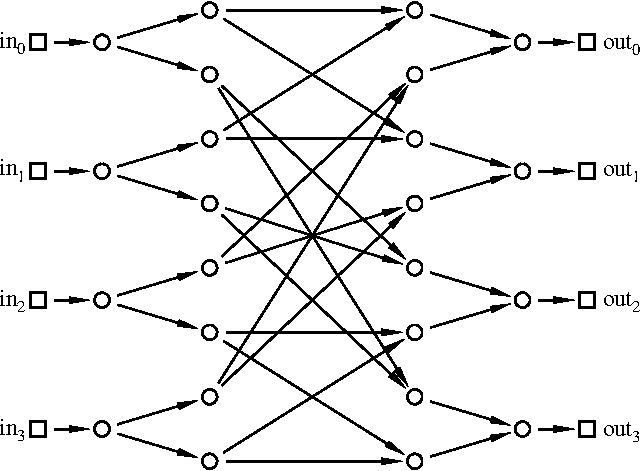
\includegraphics[scale=1]{binnet}
\end{figure}
}

\ppart{} Fill in the table, and explain your entries.

{\large
\[
\begin{array}{c|c|c|c}
\text{\# switches} &
\text{switch size} &
\text{diameter} &
\text{max congestion} \\ \hline
&&&\\ \hline
\end{array}
\]
}


\solution{
{\large
\[
\begin{array}{c|c|c|c}
\text{\# switches} &
\text{switch size} &
\text{diameter} &
\text{max congestion} \\ \hline
2n(n-1)& 1 \times 2, 2 \times 1 & 1+ 2\log n & 1\\ \hline
\end{array}
\]
}

\iffalse
\begin{align*}
\text{\# switches } & = 2n(n-1)\\
\text{switch size} & = 1 \times 2, 2 \times 1\\
\text{diameter} & =  1+ 2\log n\\
\text{max congestion} & =1
\end{align*}
\fi

These formulas were gotten as follows: a binary tree with $n/2$ leaves has
$n-1$ nodes (switches), and there are $2n$ trees.

Each node of an input tree has one edge in and two out; the opposite
for nodes of output trees.

The distance from any input to any output is 1 from input to tree root,
$(\log n)-1$ from root to leaf, 1 from input leaf to output leaf, $(\log
n)-1$ from output leaf to output root, and 1 to output, for a total of $1+
2\log n$.

The path from any input to any output is unique, and paths from two inputs
to different outputs don't overlap, so at most one packet goes through any
switch.
}

\eparts

\end{problem}


\end{document}